\begin{figure}
    \begin{center}
    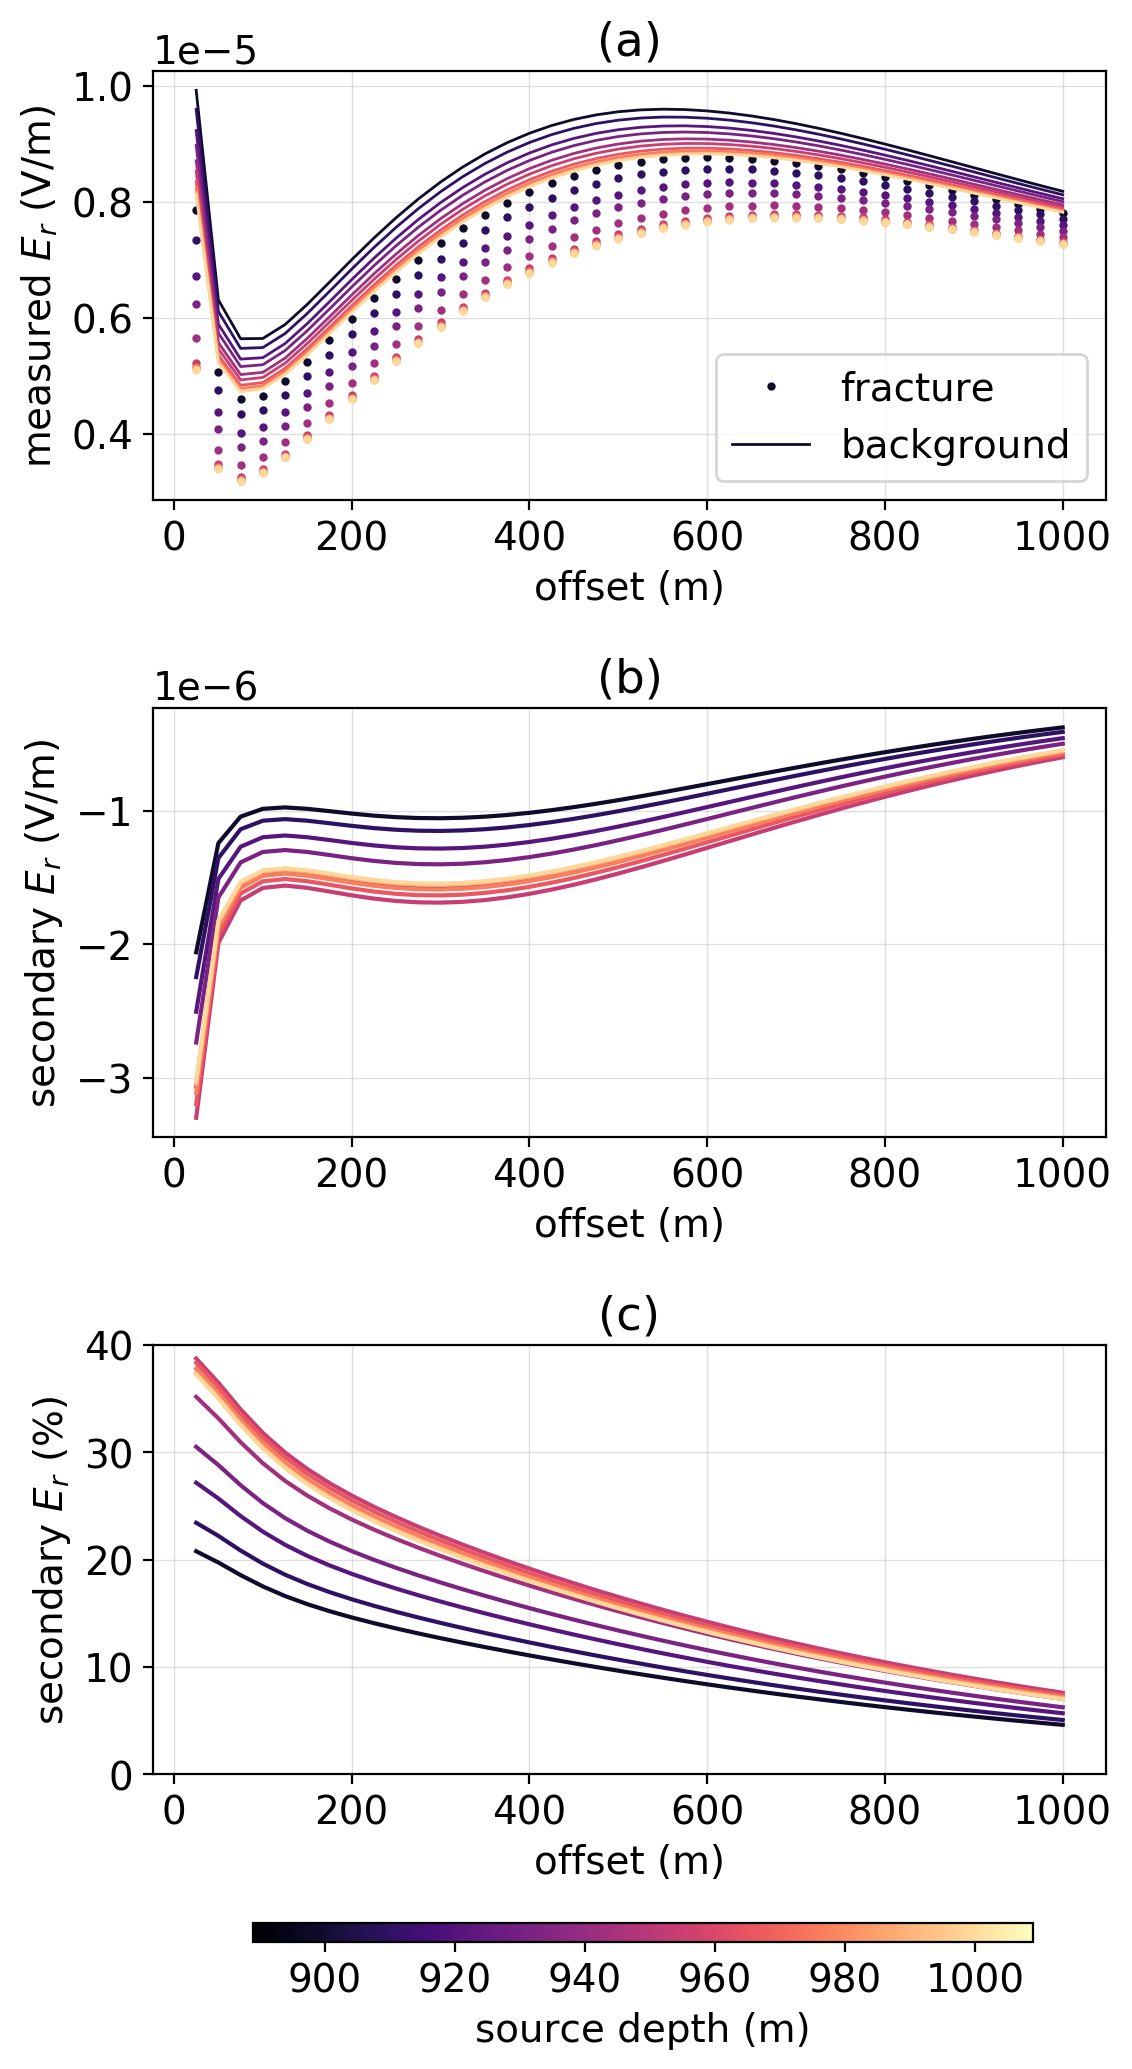
\includegraphics[width=0.6\textwidth]{figures/inversion/dc_casing_initial_data.png}
    \end{center}
\caption{
    (a) Synthetic data for the down-hole casing experiment for the background,
    prior to the fracture (solid lines), and after the fracture (dots), (b) secondary
    electric field (fracture - background), and (c) secondary electric field as a percentage
    of the primary (background). The color of the lines or dots indicates the depth of the source.
}
\label{fig:dc_casing_initial_data}
\end{figure}
